\chapter{Arquitectura de la solución}
\label{cap:arquitectura}

\section{Arquitectura}

\begin{figure}[H]
  \centering
  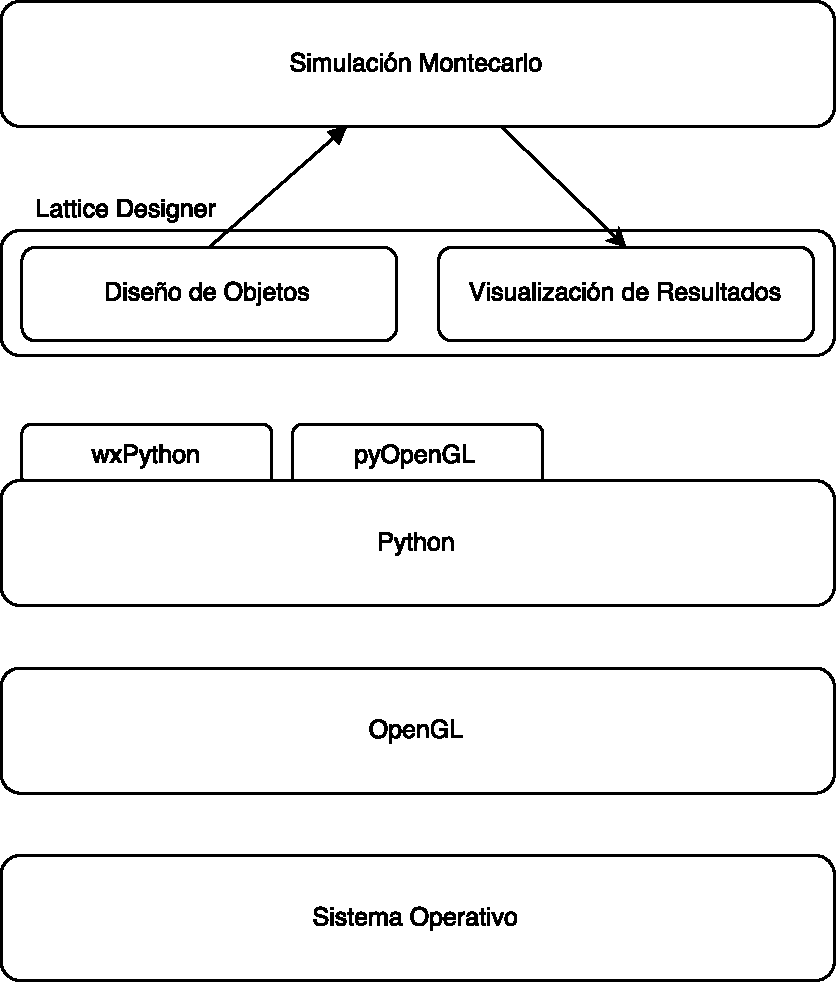
\includegraphics[scale=.7]{images/arquitectura}
  \caption{\em Diagrama de la arquitectura de la solución.}
\end{figure}

\subsection{Sistema Operativo}

Si bien la aplicación fue desarrollada íntegramente en Mac OS X, y es por lo tanto el sistema operativo oficial de la presente memoria, todo el sistema fue desarrollado pensando en ser eventualmente multi-plataforma, sin que esta portación a distintos Sistemas Operativos tenga mayores complicaciones, más allá de los problemas que uno pueda encontrar por la distinta estructura de estos. Para esto tanto la elección del lenguaje de programación como de las distintas bibliotecas usadas fueron hechas teniendo el cuenta que deben poder ser ejecutados en los 3 sistemas operativos más usados, OS X, Windows y Linux.

\subsection{OpenGL}

Como parte importante del software es su capacidad de representar gráficamente en 3D tanto los átomos de un objeto diseñado como los resultados de las simulaciones era necesario buscar una biblioteca de procesamiento gráfico 3D que fuera realmente multi-plataforma, tanto a nivel de sistema operativo como de tarjetas gráficas. Debido a esto se eligió el estándar OpenGL, el cuál tiene implementaciones tanto para Windows, OS X y Linux, además de ser el estándar de la industria para gráficos 2D y 3D \citep{website:AboutOpenGL}, esto permite tener una gran comunidad activa lo que a su vez se traduce en una gran cantidad de documentación al respecto.

La especificación del estándar OpenGL era dirigido por el consorcio independiente \emph{OpenGL Architecture Review Board} hasta el año 2006, cuando se decidió transferir esta responsabilidad al \emph{Khronos Group} \citep{website:OpenGLARB}, un consorcio formado por distintas organizaciones, tanto empresariales como académicas, quienes manejan múltiples estándares de la industria como \emph{OpenGL ES}, \emph{OpenCL} y \emph{WebGL} \citep{website:KhronosGroup}.

\subsection{Python}

Para el lenguaje de programación se barajó inicialmente la opción de C++ por las ventajas que conlleva trabajar a bajo nivel, no obstante debido a su inclinada curva de aprendizaje y complejidad se decidió usar Python, ya que era un lenguage que también cumple con las características necesarias para este desarrollo, como el ser multi-plataforma, y tener a disposición bibliotecas de manejo gráfico como su compatibilidad con la API OpenGL, de tal forma de centrar la complejidad del proyecto en las representaciones 3D.

Python es un lenguaje de programación de alto nivel, interpretado y orientado a objetos, desarrollado durante el año 1990 por Guido van Rossum, aunque actualmente es de código abierto y mantenido por su comunidad, la que es liderada por la \emph{Python Software Foundation}, quienes además resguardan los derechos de este.

Algunas de las características más conocidas de Python es su fácil sintaxis y su gran biblioteca estándar, la que cubre áreas como Protocolos de comunicación, Ingeniería de software e Interfaces de Sistema Operativo \citep{pythonFeatures}.

Durante el desarrollo se la aplicación se usaron distintas bibliotecas, siendo las dos más importantes wxPython y pyOpenGL.

\subsubsection{wxPython}

wxPython es una biblioteca de python que permite usar de forma nativa wxWidgets, un set de herramientas de código abierto, escrita en C++ y inicialmente escrito por Julian Smart y actualmente mantenida por la comunidad que permiten crear interfaces gráficas en distintas plataformas como Windows, OS X, iOS, Linux, entre otros. En la memoria presentado wxPython maneja todas las interacciones de los usuarios, además de casi todas las interfaces gráficas con excepción de los \emph{canvas} de OpenGL.

\subsubsection{pyOpenGL}

pyOpenGL es una biblioteca que permite la programación en OpenGL directamente desde python, es multiplataforma y totalmente compatible con la biblioteca de interfaz gráfica usada (wxPython). Uno de los sub-paquetes de pyOpenGL usado en esta memoria es GLUT, la que permite crear fácilmente ciertos objetos en OpenGL, como esferas o conos, de tal forma de no tener que programar estos a partir de triángulos, como sería si se usara OpenGL puro.

\section{MolDesigner}

MolDesigner es el software desarrollado en esta memoria, el cual permite a científicos generar objetos sobre los cuales se simulará la aplicación de campos electromagnéticos y la visualización de resultados generados por la simulación. Esta herramienta está pensada para ser usada por estudiantes del doctorado de física de la Universidad de Santiago de Chile, no obstante la aplicación que ejecuta la simulación es usada por diversas organizaciones académicas, por lo que este software pretende ser un aporte a la comunidad científica en general.

Durante el desarrollo se puso especial énfasis en la experiencia de usuario, de tal forma que cualquier científico que tenga acceso a esta aplicación sea capaz de usarlo sin la necesidad de un entrenamiento, por este motivo el software tiene todos sus textos en inglés.

La aplicación tiene dos funcionalidades claramente definidas, el diseño de objetos y la visualización de resultados.

\subsection{Diseño de objetos}

Para el desarrollo de esta funcionalidad se usó como base el sistema de diseño de objetos actual, basado en un mapa de bits, explicado en la sección \ref{intro:procesoactualmapa} de esta memoria, pero con la finalidad de que el proceso completo sea ejecutado en la misma aplicación disminuyendo con esto la probabilidad de errores que se puedan producir.

Dentro de las entradas de esta funcionalidad están tanto el mapa de bits, mediante una grilla binaria, como los distintos parámetros físicos asociados al objeto, como el tipo de estructura cristalina, la constante de red y el número de capas, entre otros. Además se le ofrece al usuario mucha información dinámica, es decir, que va cambiando en base a los parámetros de entrada, como por ejemplo la constante de escalamiento.

\begin{figure}[H]
  \centering
  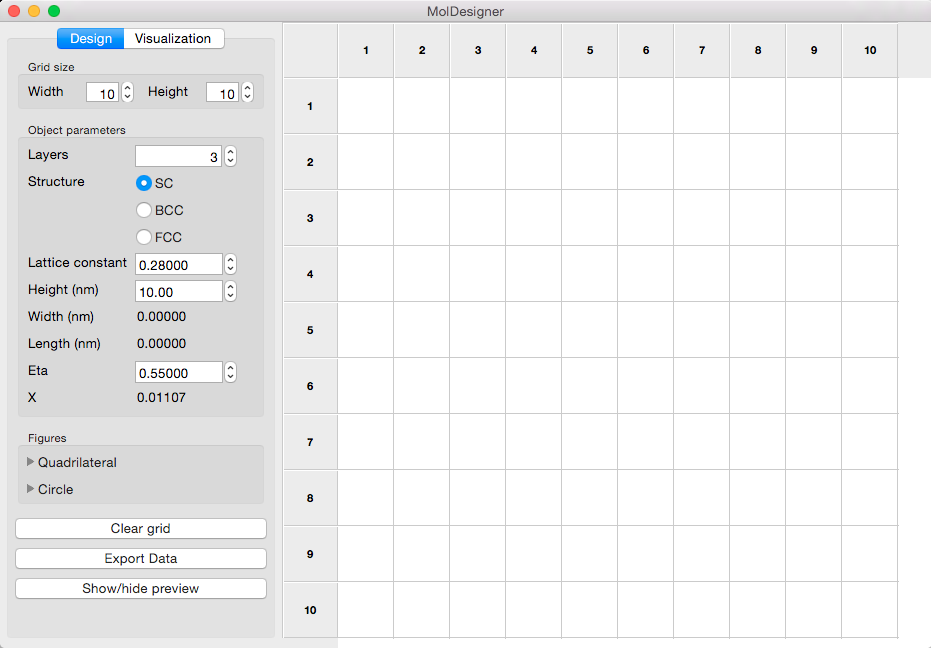
\includegraphics[scale=.45]{images/softwareDiseno}
  \caption{\em Vista de diseño de objetos del software}
\end{figure}

Una de las características del diseño es la posibilidad de crear imágenes pre-definidas en base a dimensiones entregadas por el usuario, de esta forma se pueden crear cuadriláteros definiendo su ancho y alto o circunferencias con un radio específico, una vez ingresados los parámetros solo es necesario hacer click en la posición de la grilla donde se quiere dibujar.

El software permite también al usuario ver de forma inmediata la visualización 3D del objeto que se está creando con colores identificando sus distintos tipos de partículas, permitiendo comprobar de manera rápida y fácil si efectivamente el diseño es el deseado.

\begin{figure}[H]
  \centering
  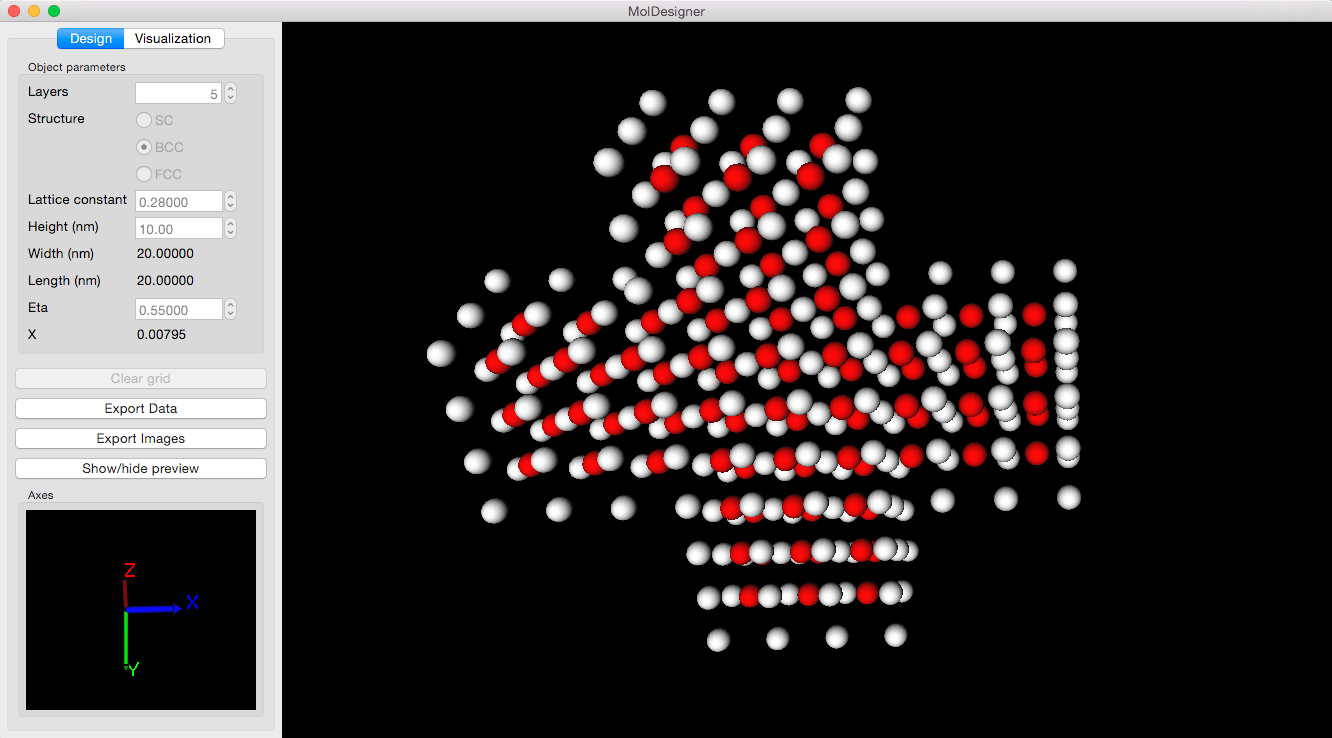
\includegraphics[scale=.35]{images/softwareDisenoPrevisualizacion}
  \caption{\em Previsualización de un objeto diseñado}
\end{figure}

Una vez confirmado que el objeto diseñado es el deseado es posible exportar directamente las imágenes del diseño y los ejes coordenados para referencia, como el archivo que servirá como entrada para el software de simulación. A diferencia del proceso actual, donde el archivo exportado debe ser modificado para poder ser usado, en este caso los datos exportados puedes ser usados inmediatamente para ejecutar una simulación.

\subsection{Visualización de resultados}

La segunda funcionalidad se basa específicamente en los requerimientos de los \emph{stakeholders}, sin tener un proceso actual como base, ya que esta es la gran debilidad que tienen actualmente.

Dentro de las características de esta funcionalidad está el ver y exportar el estado de la simulación en un tiempo \emph{t}, esto incluye los vectores de campo magnético, la curva de histéresis del campo magnético y los ejes coordenados para referencia, de forma de poder publicar sus resultados fácilmente.


\begin{figure}[H]
  \centering
  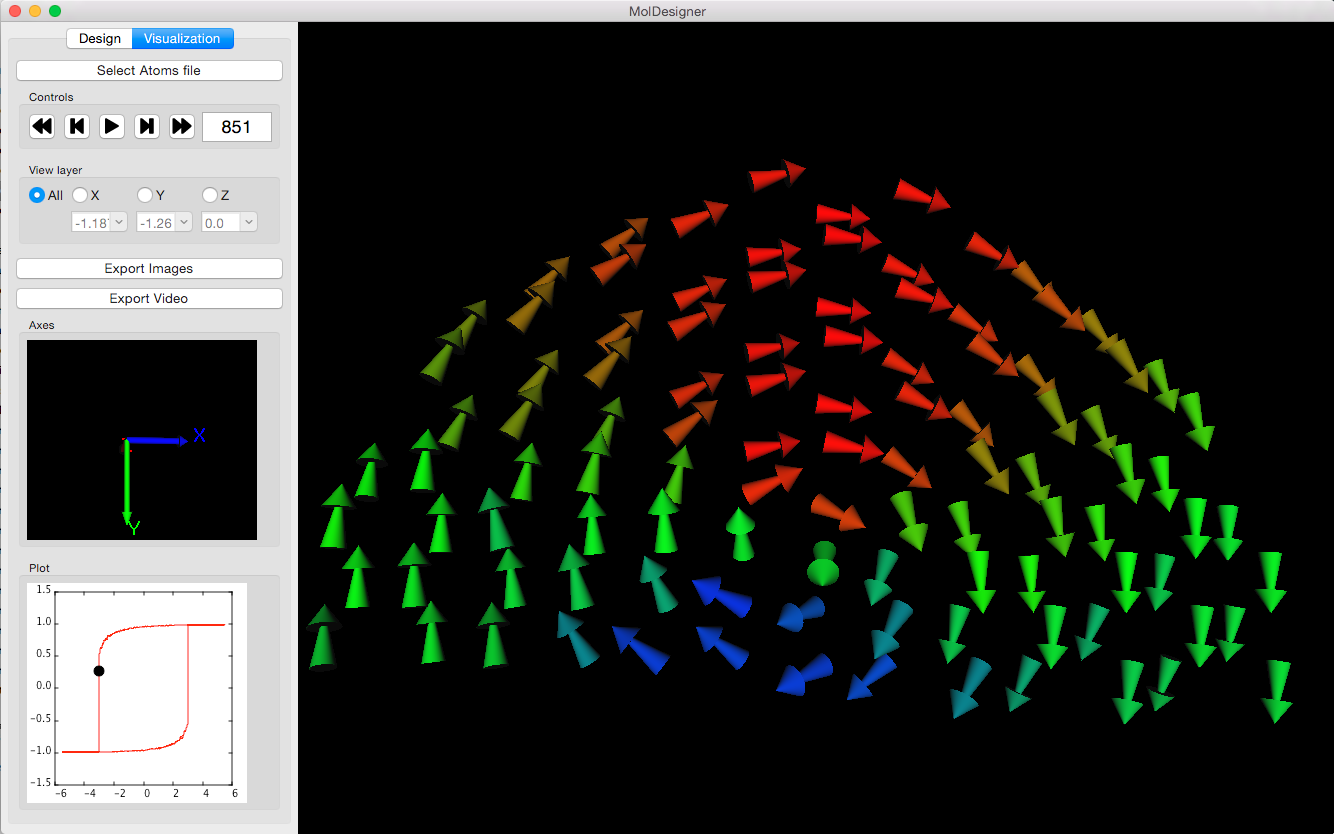
\includegraphics[scale=.3]{images/softwareVisualizacionPantalla}
  \caption{\em Pestaña de visualización de resultados en t = 851}
\end{figure}


\begin{figure}[H]
  \centering
  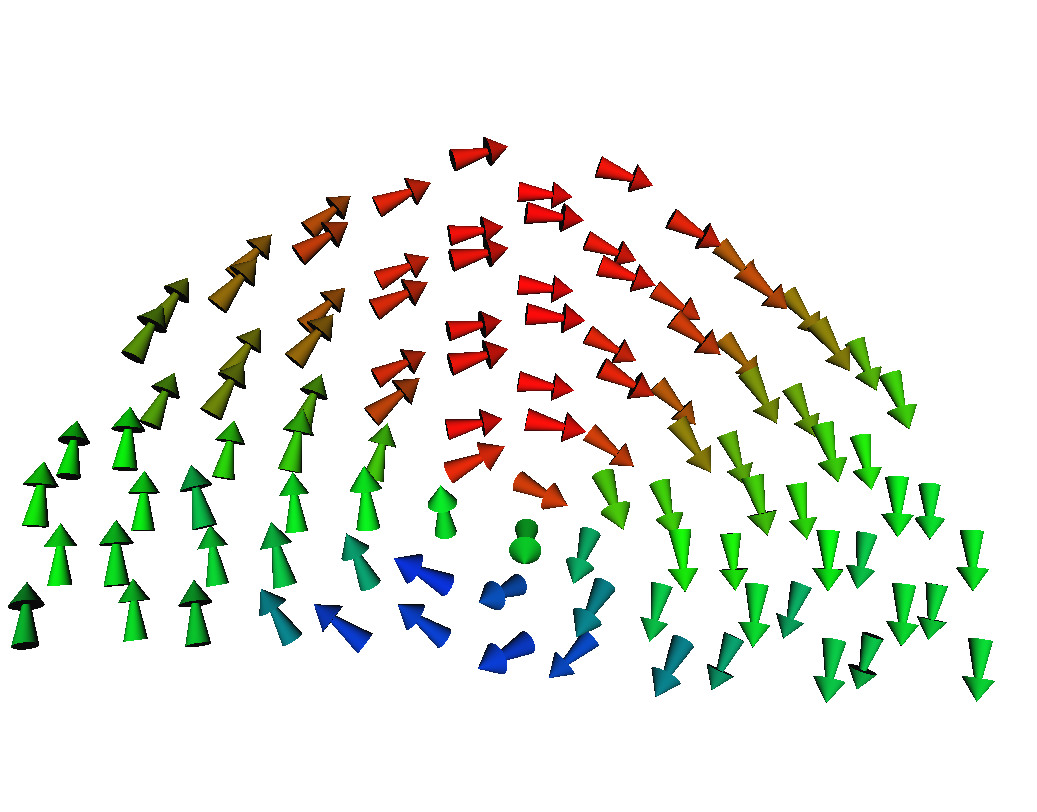
\includegraphics[scale=.3]{images/softwareVisualizacionVectors}
  \caption{\em Imagen de vectores exportada para publicación}
  \label{fig:vectors}
\end{figure}


\begin{figure}[H]
  \centering
  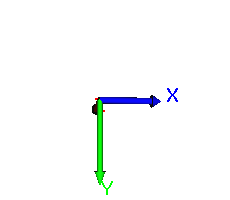
\includegraphics[scale=.6]{images/softwareVisualizacionAxes}
  \caption{\em Imagen de ejes de referencia exportada para publicación}
\end{figure}


\begin{figure}[H]
  \centering
  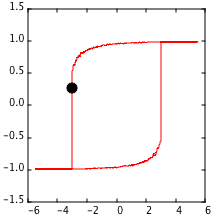
\includegraphics[scale=.6]{images/softwareVisualizacionPlot}
  \caption{\em Imagen de curva de histéresis exportada para publicación}
\end{figure}

Otras características disponibles es la asignación de colores para cada vector según uno de sus componentes, usando una escala de colores de azul a rojo, en el caso de la imagen \ref{fig:vectors} el máximo valor de $\hat{i}$ será rojo y el mínimo será azul, esto permite identificar rápidamente una tercera dimensión en una imagen 2D y también los vortex que se generan.

También es posible ver la variación de los vectores a través del tiempo como video y luego exportarlo de tal forma de que este pueda ser usado fácilmente en conferencias donde se divulguen los resultados.

Cabe notar que todas las características anteriores pueden ser ejecutadas mientras se visualiza solo una de las múltiples capas en la que se puede dividir el objeto, en base a cualquier eje.

\begin{figure}[H]
  \centering
  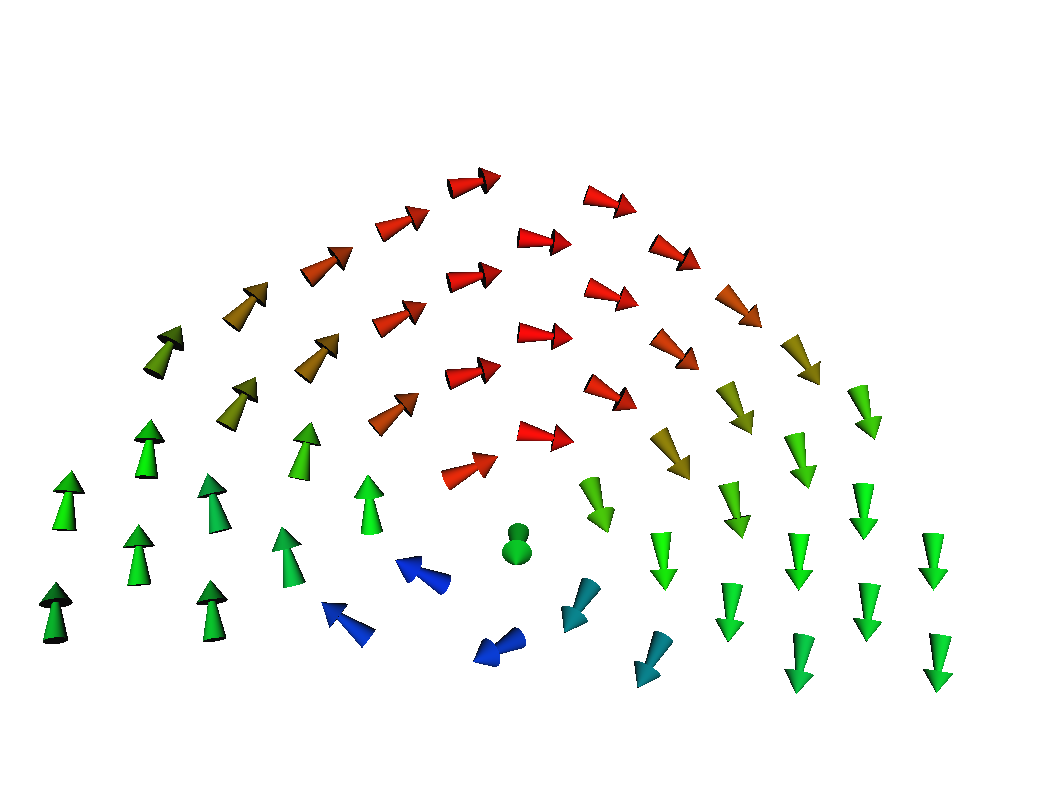
\includegraphics[scale=.3]{images/softwareVisualizacionVectorsZ}
  \caption{\em Estado de la simulación para t = 851 solo para la capa Z = 0}
\end{figure}


\begin{figure}[H]
  \centering
  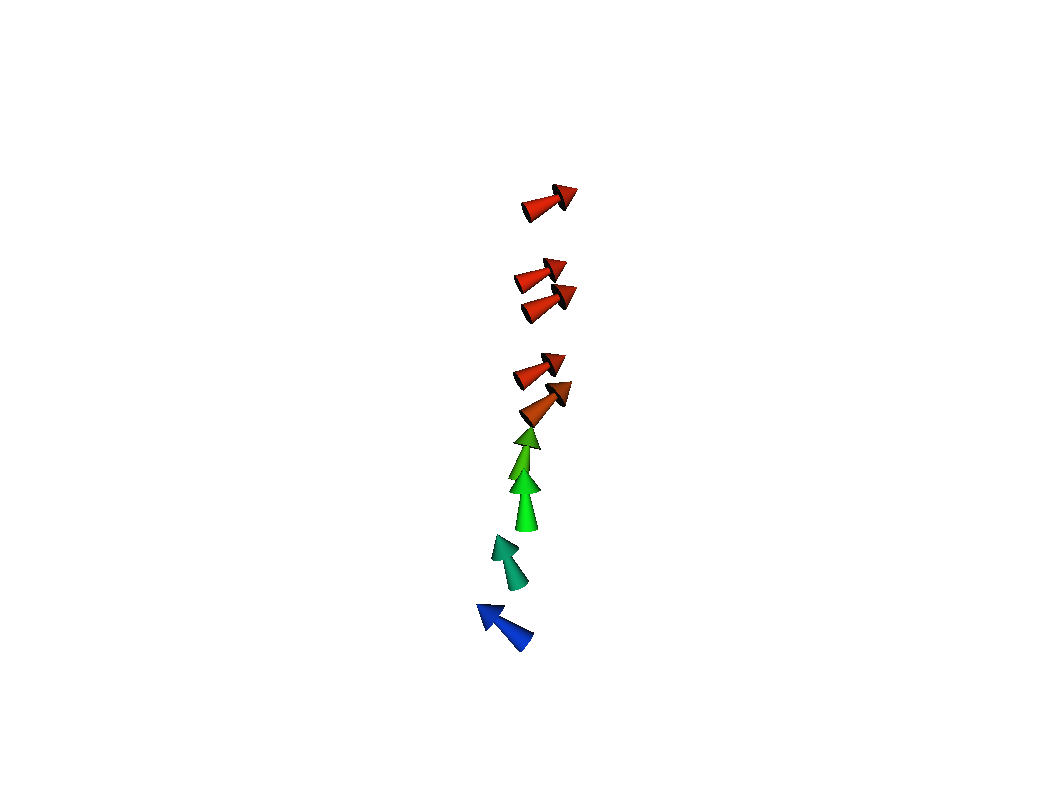
\includegraphics[scale=.3]{images/softwareVisualizacionVectorsX}
  \caption{\em Estado de la simulación para t = 851 solo para la capa X = -0.395}
\end{figure}



\section{Clases}

Para el desarrollo de la aplicación se usó el lenguaje Python, dividiendo la aplicación en clases que se pueden categorizar de la siguiente forma:

\subsection{Clases visuales}

\subsubsection{MolDesigner}
Esta es la clase principal del programa, ya que es la encargada de iniciar el programa, cargando todas las dependencias necesarias para su ejecución, pero principalmente tiene la lógica de la parte visual del \emph{software}, es decir, de la creación y distribución en pantalla de los distintos elementos visuales, como ventanas, botones, campos de texto, etc., además de la interacción del usuario con estos. Cada reacción a una acción ejecutada sobre estos elementos es orquestada por esta clase.

\subsubsection{BitmapGrid}
La clase BitmapGrid es la encargada de manejar la grilla con la cuales los científicos diseñarán los objetos sobre los cuales se simulará, para esto se basa en la biblioteca \emph{wx.grid} de \emph{wxPython}, una implementación de una planilla de cálculos tipo \emph{excel}, la cual es modificada para no poder ser editada y que las distintas acciones del \emph{mouse} sobre esta (click, seleccionar fila o columna, seleccionar un rango de celdas, etc.) generen cambios en el color de fondo de cada celda, pudiendo este ser negro o blanco, transformando esta planilla de cálculos en un mapa de bits binario.

Entre las características de este mapa de bits se encuentra la capacidad de crear figuras predefinidas rápidamente, por ejemplo, se puede dibujar un cuadrilátero indicando el ancho, el alto y seleccionando la esquina superior derecha de esta figura. También es posible crear un círculo indicando el radio que tendrá este y su centro.

\begin{figure}[H]
  \centering
  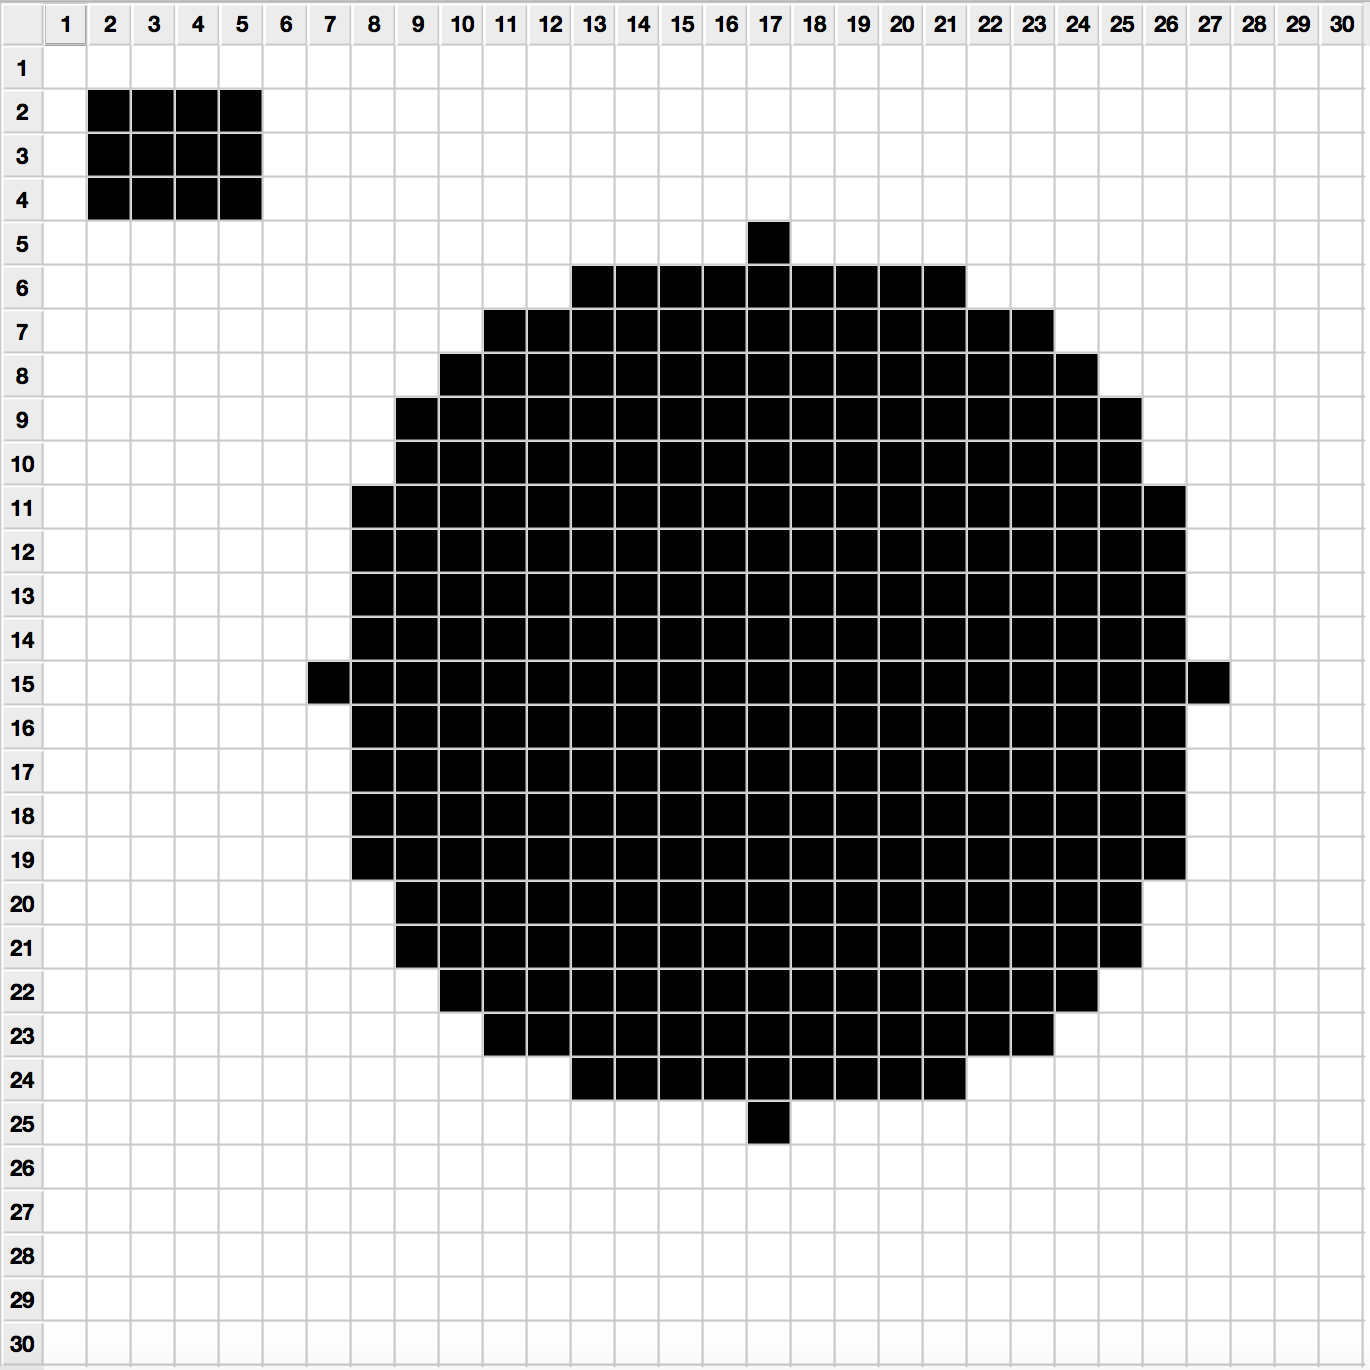
\includegraphics[scale=.5]{images/bitmapGrid}
  \caption{\em Mapa de bits binario con 2 figuras pre-diseñadas.}
\end{figure}

\subsection{Clases 3D}

Estas clases son las encargadas de manejar los distintos \emph{canvas} que se usan en el \emph{software}, tanto para la visualización del diseño y del resultado de la simulación, como para ayudas referenciales para los científicos.

\subsubsection{AtomCanvas}

La clase AtomCanvas es la más importante con respecto a la visualización 3D, ya que es la encargada de mostrar en pantalla tanto el diseño de los objetos sobre los cuales se correrá la simulación como los resultados de estas usando OpenGL. En el desarrollo de esta se puso énfasis en la optimización, pudiendo mostrar sin mayores demoras más de 20.000 átomos, para tener una idea un sistema promedio analizado por los científicos usa 3.000 átomos (TODO: CONFIRMAR).

Otra de las tareas de esta clase es manejar las distintas interacciones del usuario, tanto con el teclado como con el \emph{mouse} con las representaciones en 3D, como rotaciones, movimientos y \emph{zoom}.

Para la visualización del diseño se usan esferas de distintos colores, representando cada uno de los distintos tipos de átomos que pueden haber según la estructura cúbica elegida. En las siguientes imágenes se representan una estructura de 5x5, con 3 capas, siendo solo diferente la estructura cúbica elegida.

\begin{figure}[H]
  \centering
  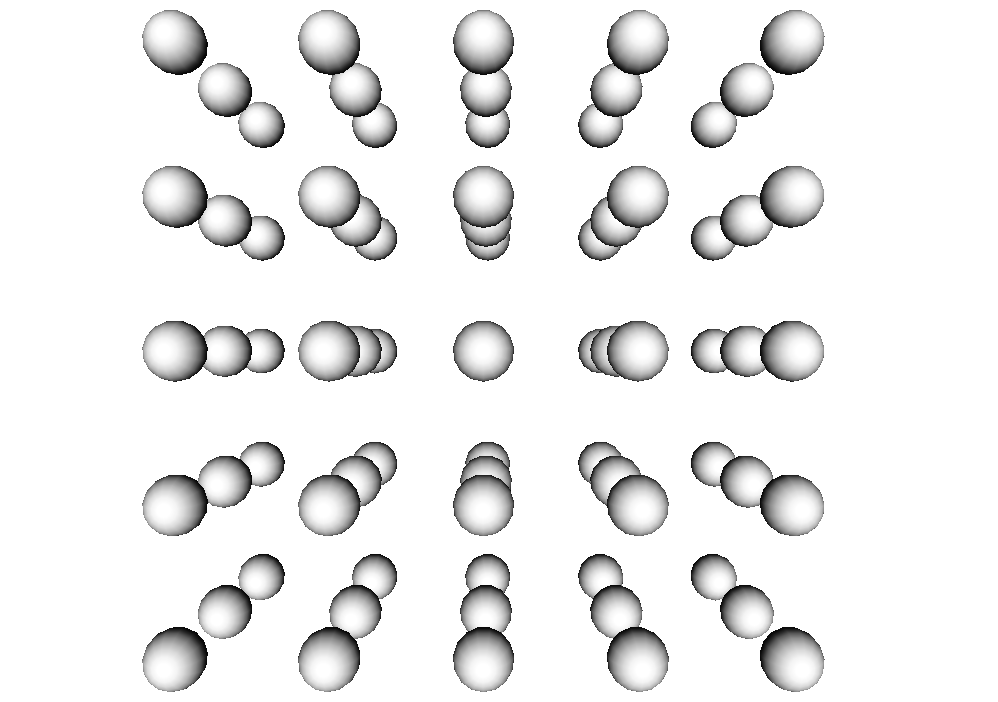
\includegraphics[scale=.3]{images/atomCanvas-SC}
  \caption{\em En un SC todos los átomos son blancos.}
\end{figure}

\begin{figure}[H]
  \centering
  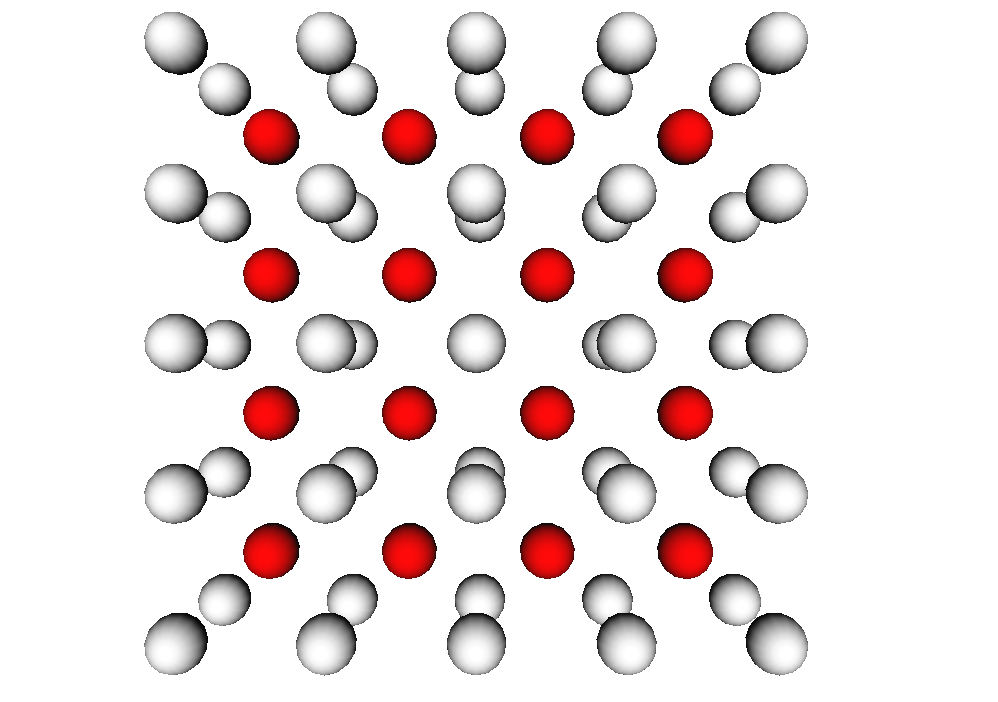
\includegraphics[scale=.3]{images/atomCanvas-BCC}
  \caption{\em En un BCC los átomos centrales son rojos.}
\end{figure}

\begin{figure}[H]
  \centering
  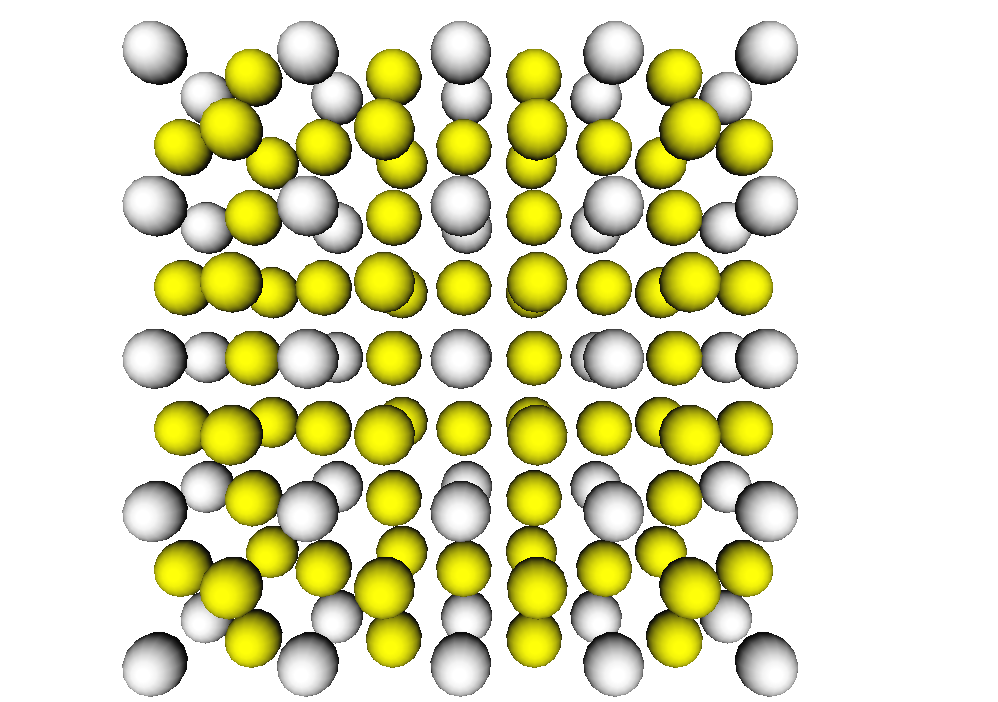
\includegraphics[scale=.35]{images/atomCanvas-FCC}
  \caption{\em En un FCC los átomos de las caras son amarillos.}
\end{figure}

En el caso de la visualización de resultados se usan flechas de colores como representación. Para asignar un color a una flecha se parte de la premisa que en tiempo t=0 el campo magnético está cargado hacia un eje, es decir, todos los vectores serán iguales, teniendo la misma magnitud, sentido y dirección, estando este paralelo a uno de los ejes del plano coordenado; además se sabe que en ese momento su magnitud es máxima. Si inicialmente todos los vectores son paralelos al eje A, se usará la componente â de cada vector para definir el color, si la componente es 0 será de color verde, si la magnitud es máxima en sentido contrario a los vectores iniciales el color será azul, si la magnitud es máxima en el mismo sentido de los vectores iniciales el color será rojo. Como se puede inferir la escala va desde azul a rojo, siendo este último color el inicial para todos los vectores.

\begin{figure}[H]
  \centering
  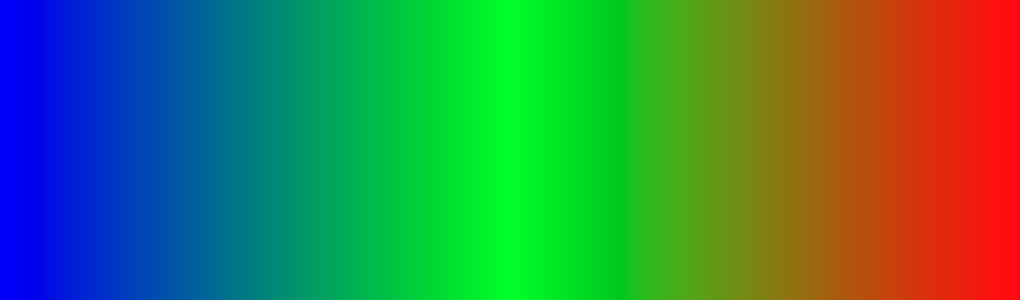
\includegraphics[scale=.4]{images/atomCanvas-colorScale}
  \caption{\em Escala de colores de azul a rojo.}
\end{figure}

\begin{figure}[H]
  \centering
  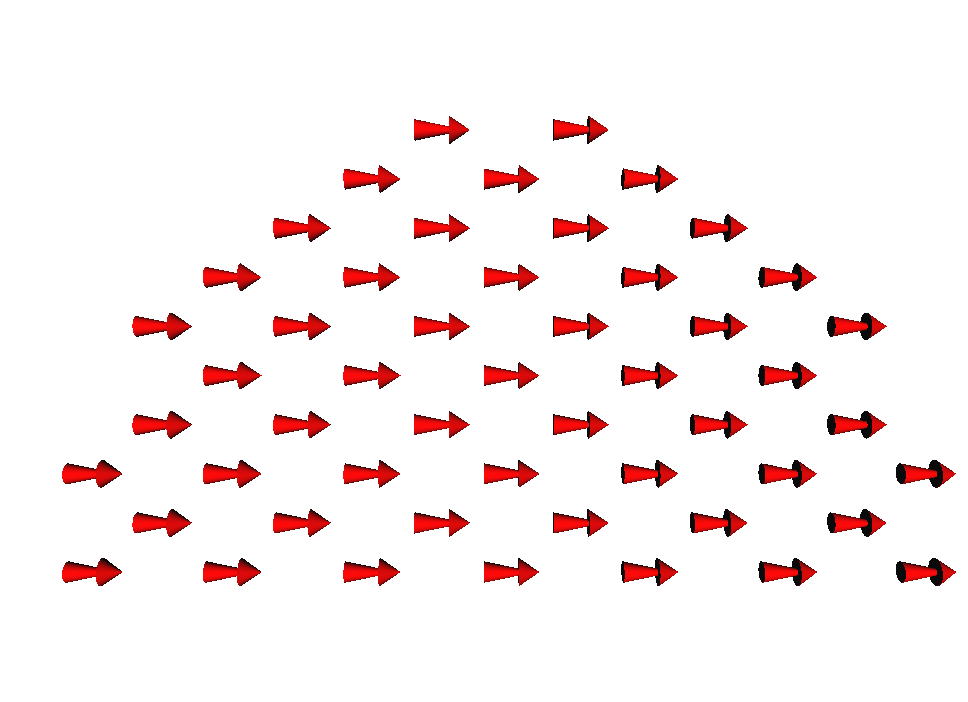
\includegraphics[scale=.3]{images/atomCanvas-vectores-inicial}
  \caption{\em Estado inicial de la visualización, con todos los vectores rojos cargados al eje X.}
\end{figure}

\begin{figure}[H]
  \centering
  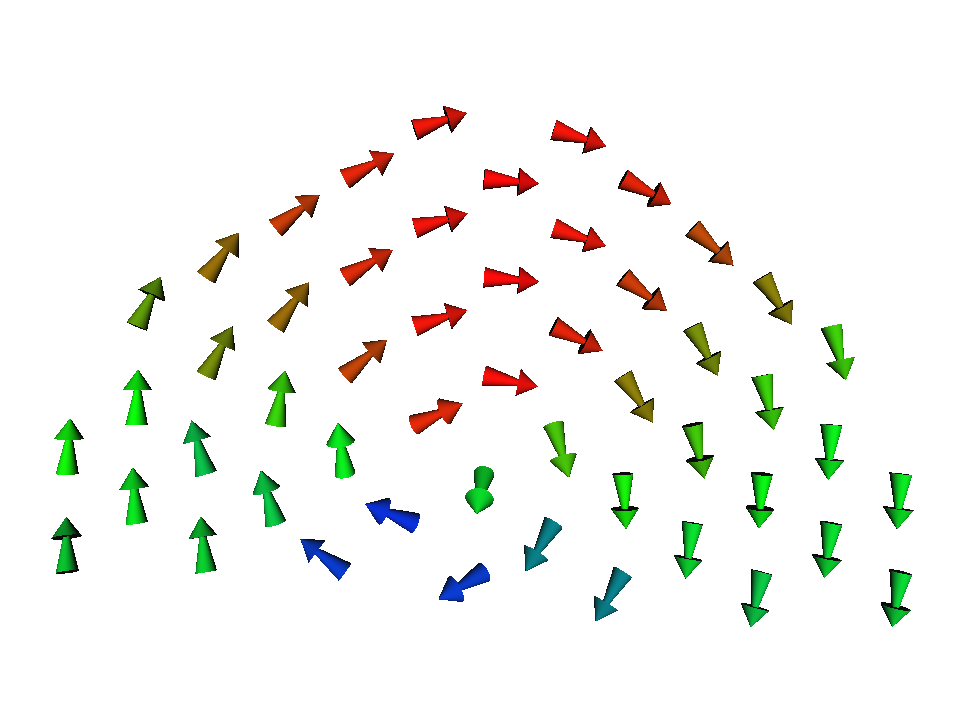
\includegraphics[scale=.3]{images/atomCanvas-vectores-colores}
  \caption{\em Vectores de distintos colores según la componente $\hat{i}$.}
\end{figure}

\subsubsection{Axes}

La clase Axes es la encargada de mostrar los ejes coordenados de los distintos canvas, tanto del de diseño de objetos como el de visualización de resultados, usando Open GL.
Cada eje se representa con su propio color, usando azul, rojo y verde para los ejes X, Y y Z respectivamente, y una etiqueta con el mismo color, de forma de hacerlo fácil de visualizar para el usuario.
Debido al diseño del \emph{software}, donde las distintas funciones del programa (diseño y visualización) se seleccionan mediante pestañas, esta clase debe ser instanciada 2 veces, ya que no es posible usar la misma instancia en ambas secciones. Estas se comunican directamente con AtomCanvas para obtener los distintos parámetros de rotación de forma que los ejes sean coherentes a la imagen mostrada.

\begin{figure}[H]
  \centering
  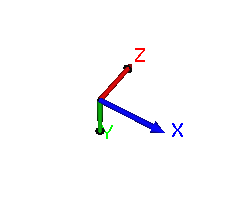
\includegraphics[scale=1]{images/axes}
  \caption{\em Representación visual de los ejes coordenados.}
\end{figure}

\subsection{Clases de cubos}

Las clases de cubos son 3 clases hermanas que calculan los átomos de un objeto que se está diseñando, todas tienen solo 2 métodos: \emph{calculate} y \emph{find\_neighborhood}, el primero se encarga de identificar todos los átomos que aplican dados los parámetros físicos como la estructura de la primera capa, luego el segundo busca, para cada átomo, todos sus vecinos inmediatos, estos parámetros son necesarios para exportar el archivo que luego servirá de entrada para la simulación.

\subsubsection{SC}
SC es la clase que maneja los cubos simples (\emph{Simple Cubic} o \emph{SC}), estas estructuras cúbicas se caracterizan por tener un átomo en cada uno de sus vértices, por lo que el cálculo de sus átomos se reduce a simplemente repetir la capa superior tantas veces como sea indicado en la entrada de propiedades físicas. Para encontrar el vecindario es necesario buscar todos los átomos que estén en las siguientes posiciones relativas [-1,0,0], [1,0,0], [0,-1,0], [0,1,0], [0,0,-1] y [0,0,1], por lo que el tamaño máximo de su vecindad es de 6 átomos.

\subsubsection{BCC}
BCC es la clase que maneja los cubos centrados en el cuerpo (\emph{Body Centered Cubic} o \emph{BCC}), que son las estructuras cúbicas que además de tener un átomo en cada vértice de los cubos tienen uno en el centro de cada uno de estos, de tal forma que en el cálculo de átomos se debe trabajar con una capa intermedia que contendrá los centros de cada cubo, de tal forma que para una estructura de 5 capas quedaría así:
\begin{center}
  \begin{tabular}{ c | l }
    \# & Capa \\
    \hline
    1 & Primaria \\
    2 & Intermedia \\
    3 & Primaria \\
    4 & Intermedia \\
    5 & Primaria \\
    \hline
  \end{tabular}
\end{center}

La regla para agregar un átomo central es que debe tener un cubo de átomos a su alrededor, en caso de que el cubo no esté completo simplemente se usarán las capas primarias:

\begin{figure}[H]
  \centering
  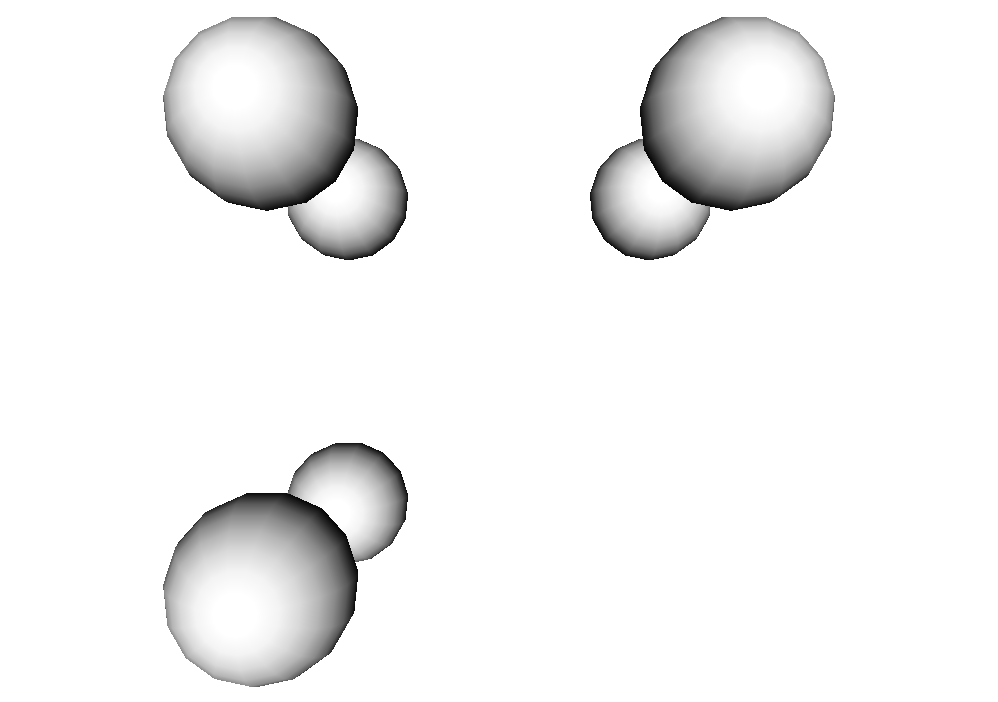
\includegraphics[scale=.3]{images/BCC-incomplete-molecule}
  \caption{\em Cubo BCC incompleto, sin átomo central}
\end{figure}

\begin{figure}[H]
  \centering
  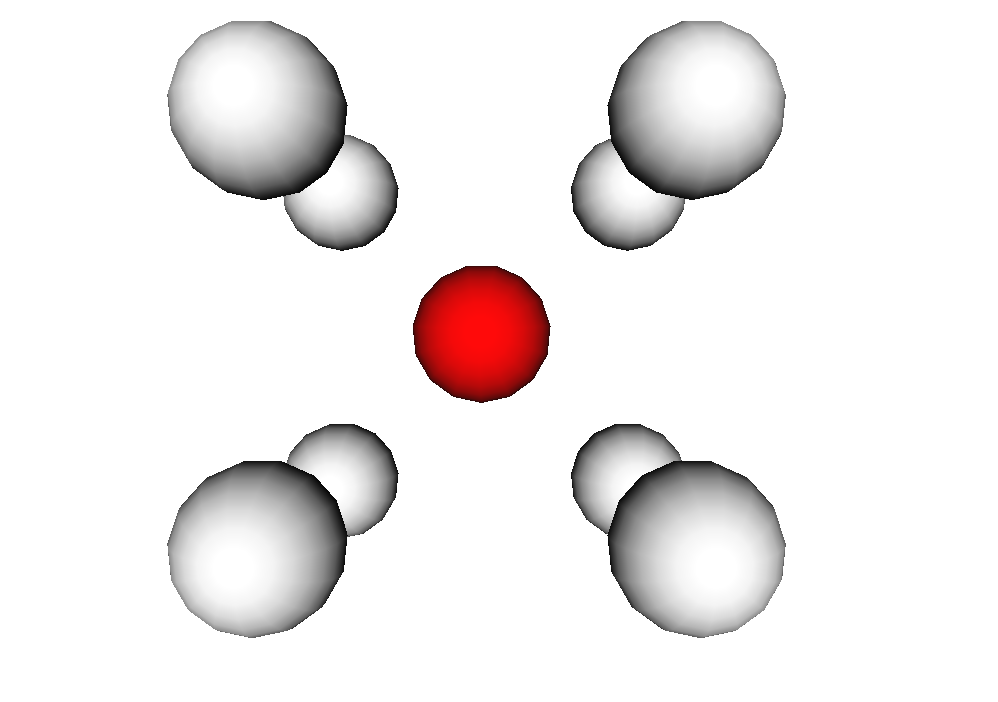
\includegraphics[scale=.3]{images/BCC-complete-molecule}
  \caption{\em Cubo BCC completo, con átomo central}
\end{figure}

En el caso de los BCC los átomos que conforman la vecindad siempre estarán en las posiciones relativas $[\pm 0.5, \pm 0.5, \pm 0.5]$, es decir, cada átomo puede tener una vecindad compuesta por hasta 8 átomos.

\subsubsection{FCC}
FCC es la clase que maneja los cubos centrados en las caras (\emph{Face Centered Cubic} o \emph{FCC}), los cuales se caracterizan por tener un átomo extra por cara además de uno en cada uno de sus vértices, por lo que además de tener que crear una capa intermedia es necesario modificar la capa primaria, es decir, la que crea el usuario usando el mapa de bits. La regla para agregar estos átomos en las caras es que esté en la diagonal creada por otros 2 átomos, en cualquier dirección. En la siguiente imagen se ve una estructura cúbica de 1x2, como en una de sus caras se forma una diagonal entre 2 átomos se agrega uno extra en una capa intermedia.

\begin{figure}[H]
  \centering
  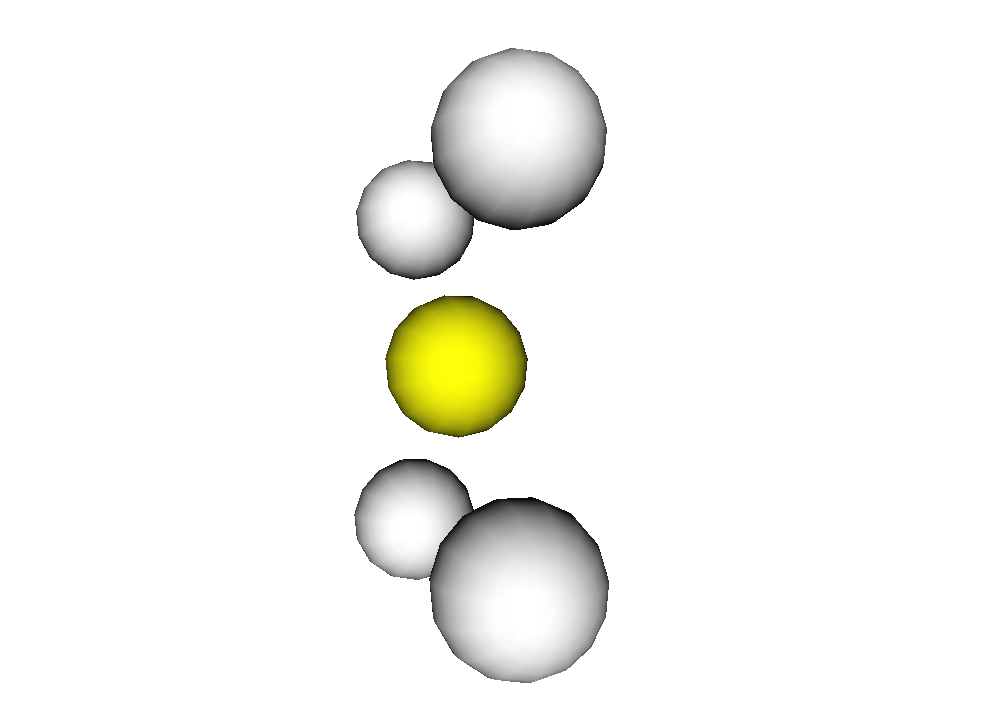
\includegraphics[scale=.3]{images/FCC-diagonal}
  \caption{\em Estructura cúbica FCC, con átomo en una de sus caras}
\end{figure}

La vecindad de estas estructuras cúbicas está dada por la posición relativa dada por $[\alpha, \beta, \gamma]$, donde:

$$ (\alpha = \pm 0.5; \beta = \pm 0.5; \gamma = 0) \vee (\alpha = \pm 0.5; \beta = 0; \gamma = \pm 0.5) \vee (\alpha = 0; \beta = \pm 0.5; \gamma = \pm 0.5)$$

Lo que en su combinatoria resulta 12 posiciones, siendo este el número máximo de átomos en una vecindad.